\documentclass[12pt]{article}

\usepackage[a4paper, total={6in, 8in}]{geometry}
\usepackage{graphicx}

\graphicspath{ {./images/} }

\title{Incendio di un porto di mare}
\author{Eugenio Barbieri Viale, Leonardo Ippoliti}
\date{4D - a.s. 2024/2025}

\begin{document}
\setlength{\parindent}{0pt}
\maketitle

\begin{figure}[ht]
    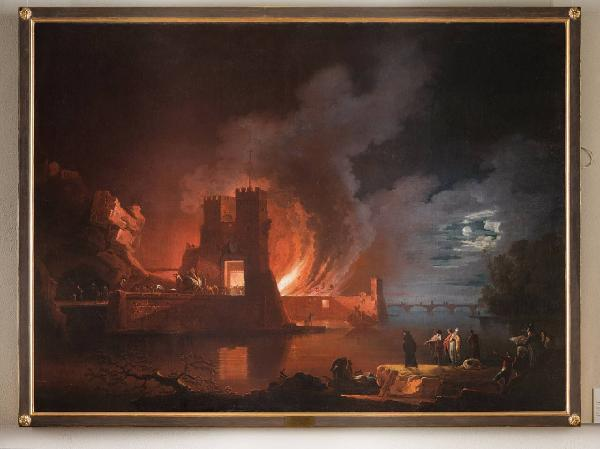
\includegraphics[scale=0.6]{dipinto}
    \centering
\end{figure}

\begin{figure}[h]
    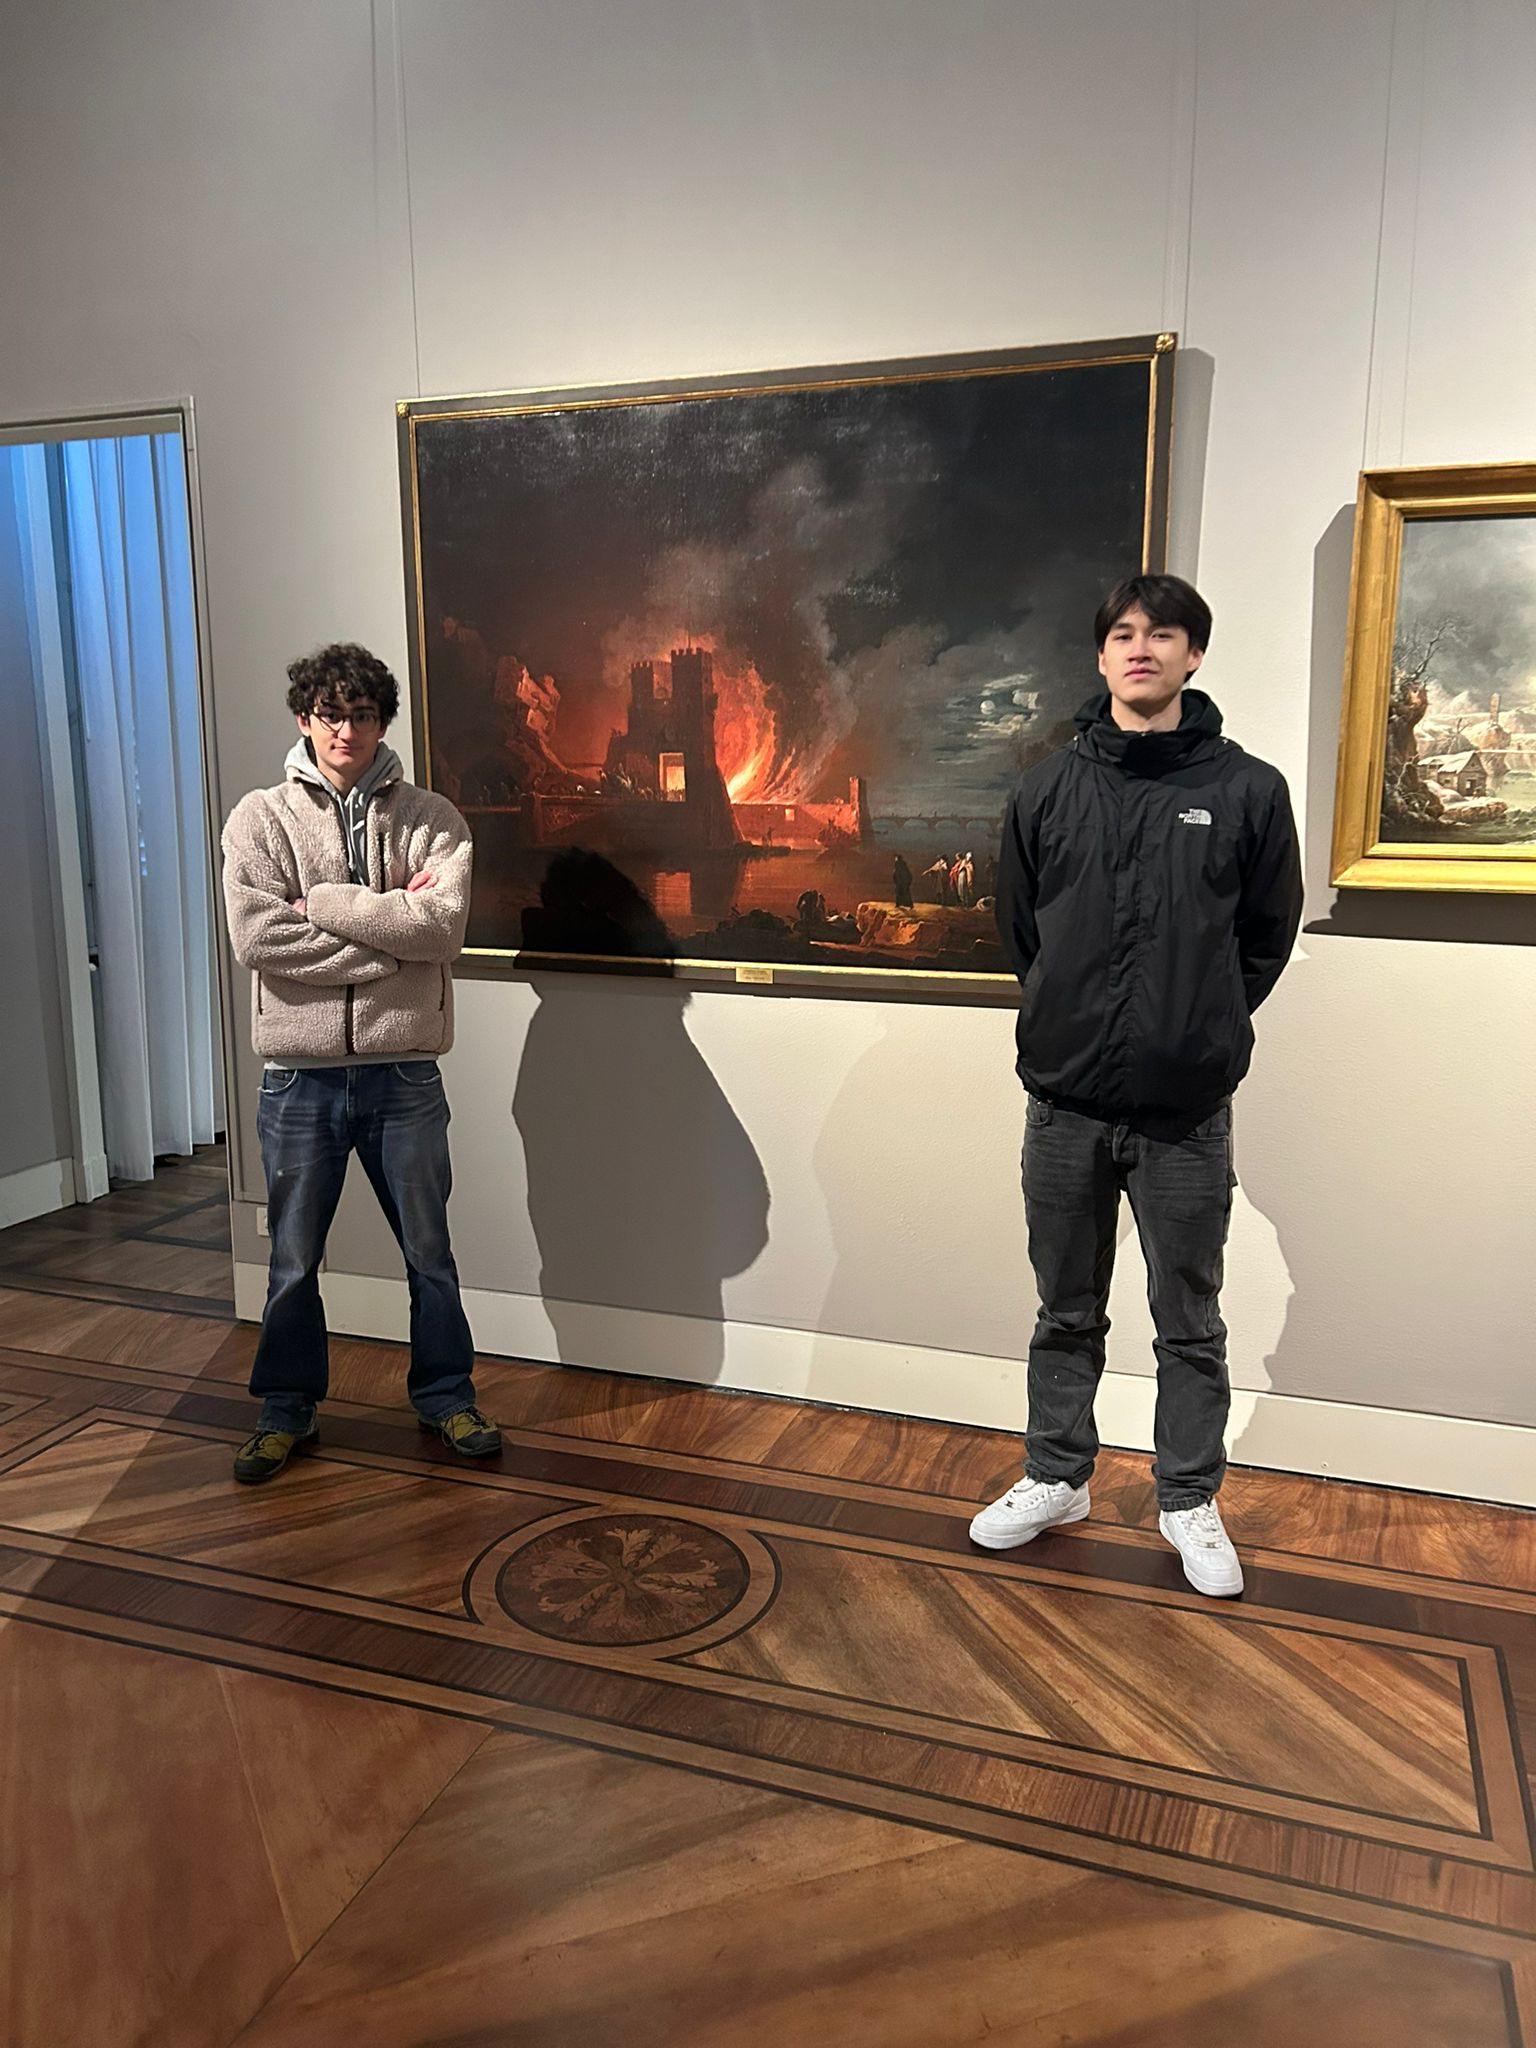
\includegraphics[scale=0.03]{selfie}
    \centering
\end{figure}

\newpage
\section*{L'artista - Francesco Fidanza}
\subsection*{Vita}
Francesco Fidanza è un pittore italiano e nasce a Roma nel 1747. Si trasferisce a Firenze nel 1793, e nell'anno 1800 a Parigi. Qui probabilmente diventa allievo di \textit{Claude Joseph Vernet}, il quale influenza la sua pittura. Il pittore francese aveva infatti realizzato numerosi dipinti di porti per conto di Luigi XV. Dopo il soggiorno francese il pittore si trasferisce a Milano, dove viene stipendiato dal vicerè \textit{Eugenio di Beauharnais}. Trascorre gli ultimi anni della sua vita nell'ozio e si indebita sempre di più, finchè non muore nel 1819.

\subsection*{Stile}
Francesco Fidanza rappresenta principalmente paesaggi marittimi e invernali e si concentra su effetti metereologici improvvisi, come tempeste o mareggiate. Caratteristico è anche il suo utilizzo del colore, attraverso il quale esprime l'irrequietezza della natura. Il pittore è infatti spesso considerato un artista preromantico.


\newpage
\section*{L'opera - Incendio di un porto di mare}

\subsection*{Informazioni}
\begin{itemize}
    \item \textit{Autore}: Francesco Fidanza
    \item \textit{Titolo}: Incendio di un porto di mare
    \item \textit{Data di esecuzione}: 1798
    \item \textit{Materiali e tecnica}: Olio su tela
    \item \textit{Dimensioni}: 170cm x 145cm
    \item \textit{Collocazione}: Milano, Galleria d'Arte Moderna
    \item \textit{Committenza}: Eugenio di Beauharnais
    \item \textit{Orientamento artistico}: Preromanticismo
    \item \textit{Genere}: Paesaggio
    \item \textit{Tema}: Un porto avvolto dalle fiamme di notte
\end{itemize}

\newpage
\section*{Analisi iconografica}
\begin{figure}[h]
    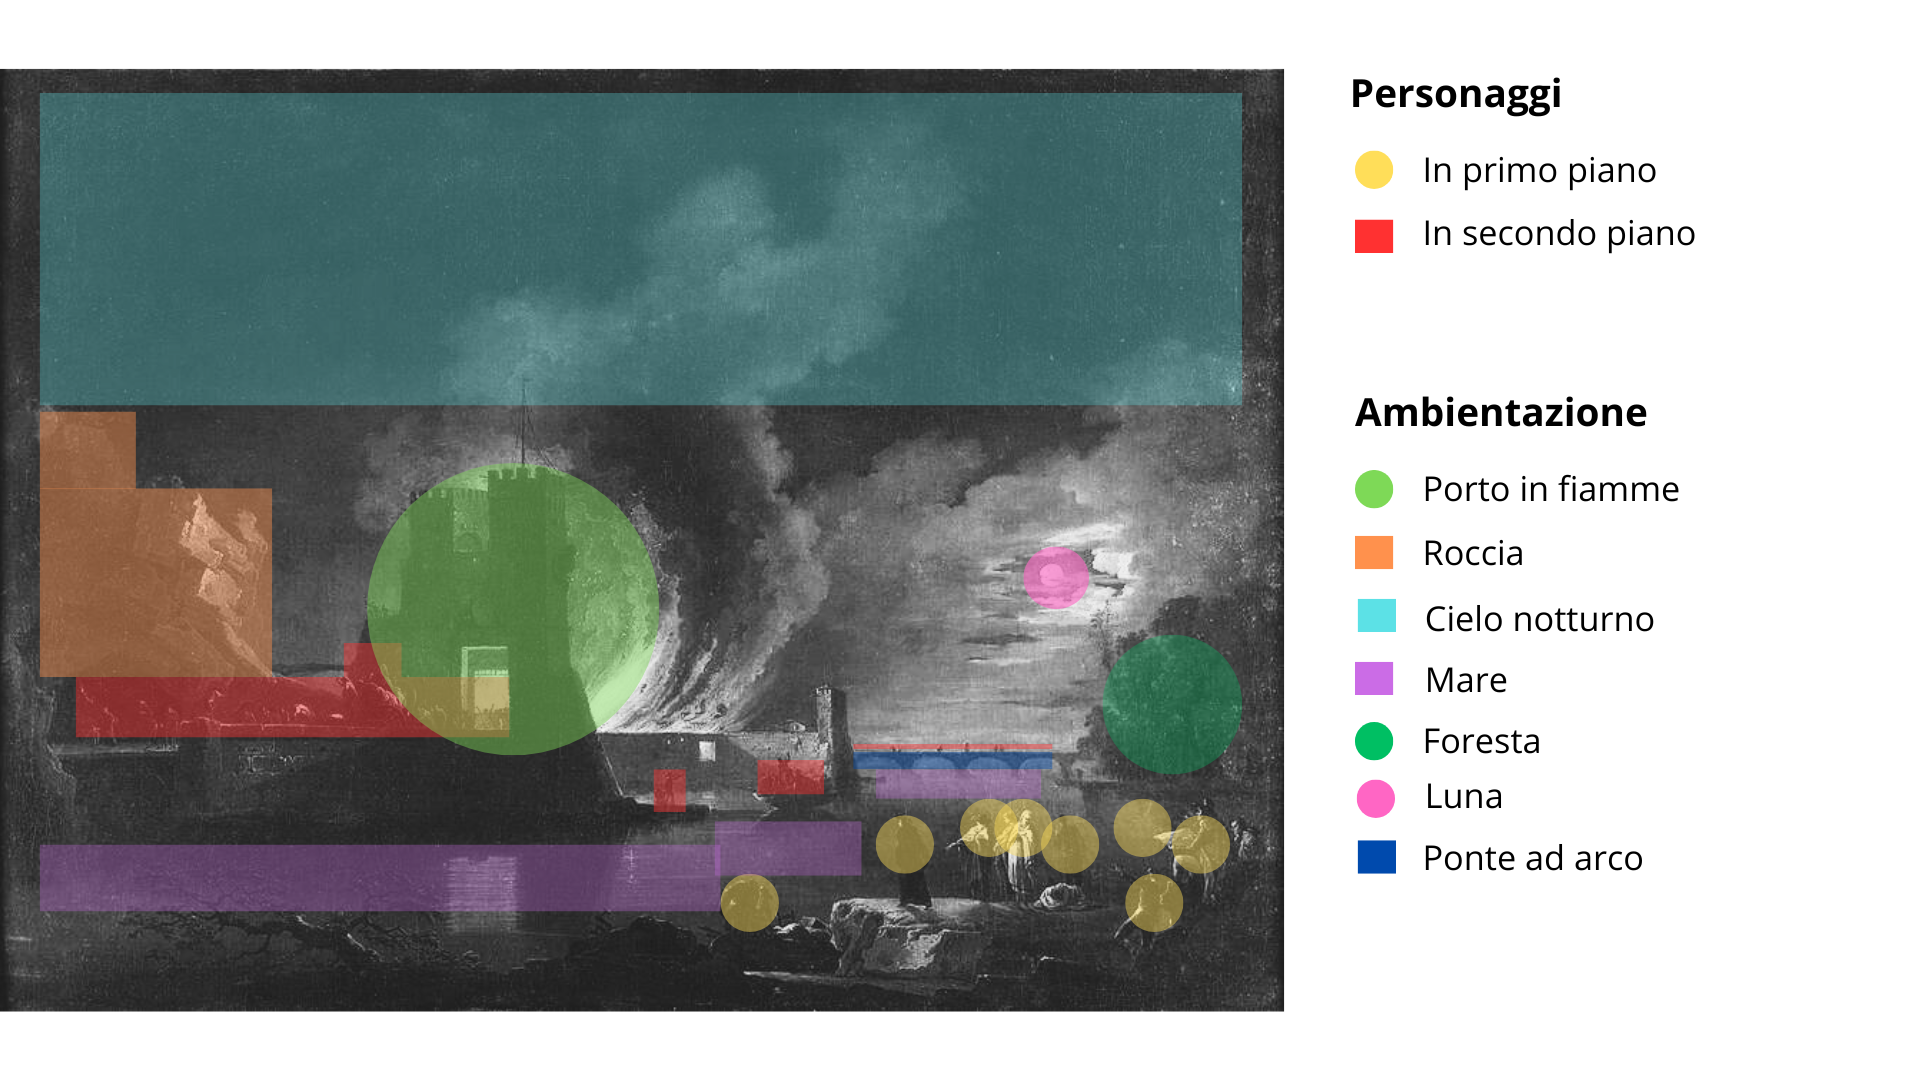
\includegraphics[scale=0.31]{analisi_iconografica}
    \centering
\end{figure}

Nell'opera le figure umane, dipinte molto piccole, perdono di rilevanza in confronto alla natura, che invece è il soggetto principale. \\
L'ingresso al porto presenta un portone ed è caratterizzato da due torrioni, sui quali si trovano dei merli guelfi.

\newpage
\section*{Analisi formale}
\begin{figure}[ht]
    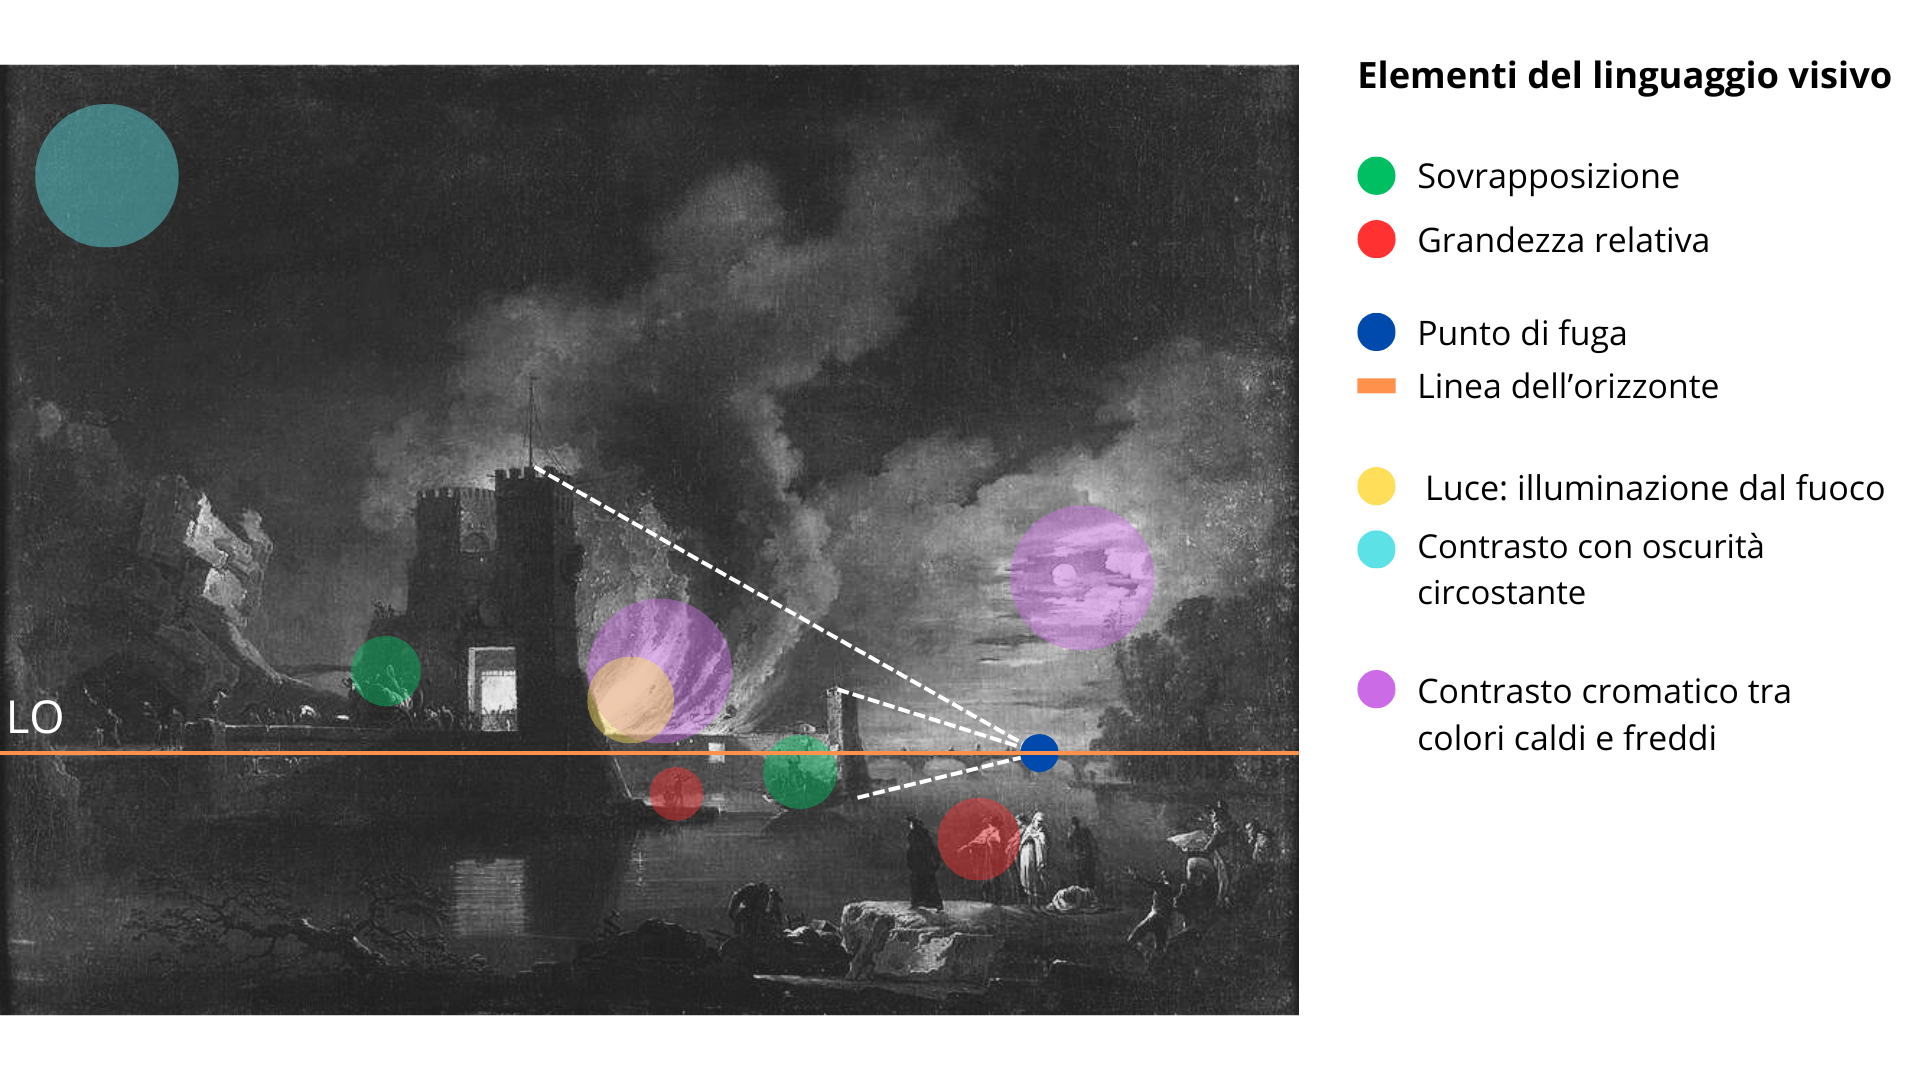
\includegraphics[scale=0.3]{analisi_formale}
    \centering
\end{figure}

Dal punto di vista formale sono presenti due contrasti. 
\begin{itemize}
    \item \textit{contrasto luce/ombra:} tra la forte luminosità del fuoco, che illumina tutta la scena, e l'oscurità circostante della notte
    \item \textit{contrasto cromatico:} tra i colori caldi dell'incendio e i colori freddi della luna e delle nuvole. L'opposizione dei colori si estende anche nel riflesso sull'acqua
\end{itemize}

\newpage
\section*{Analisi compositiva}
\begin{figure}[h]
    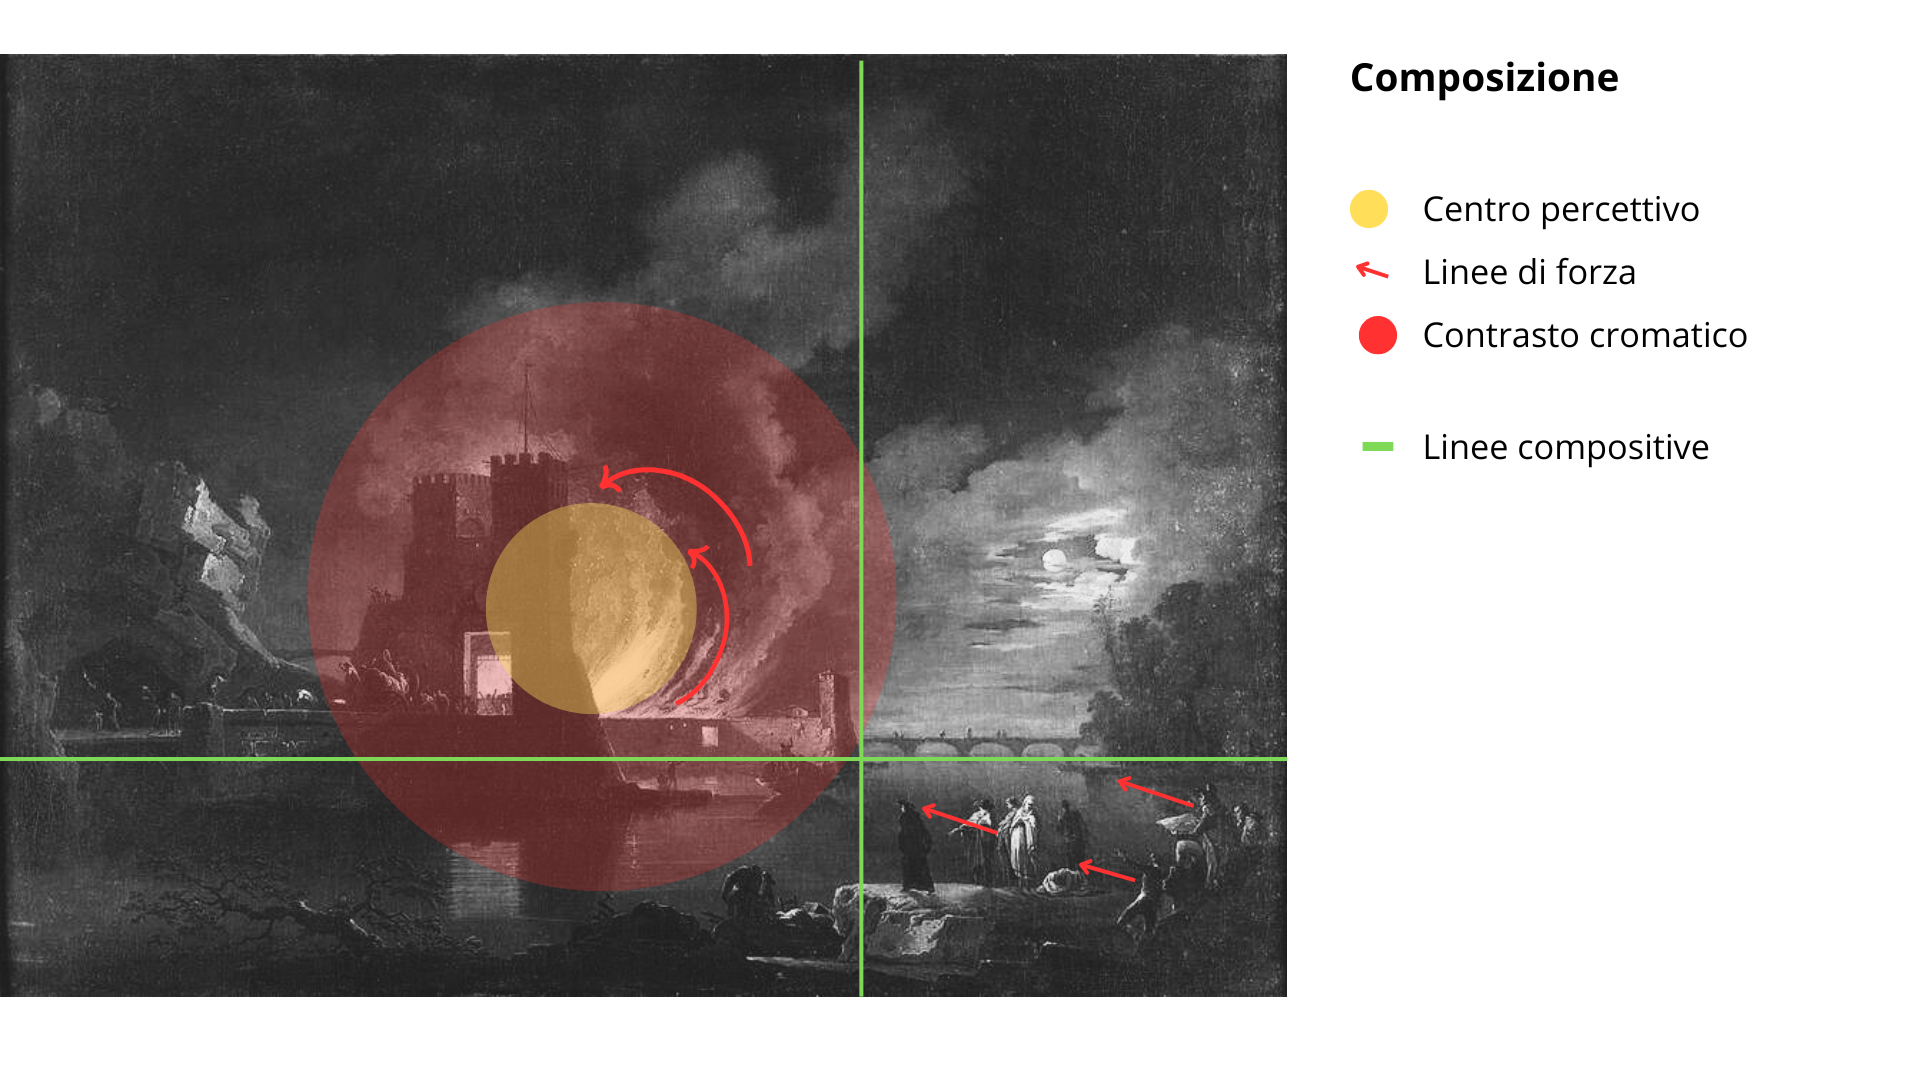
\includegraphics[scale=0.31]{analisi_compositiva}
    \centering
\end{figure}

Il centro percettivo è individuato principalmente dall'andamento curvo delle nubi di fumo e dal contrasto sia cromatico sia luminoso del fuoco.

\vspace{1em}

Sono presenti due linee compositive:
\begin{itemize}
    \item \textit{orizzontale:} separa gli elementi in primo piano da quelli in secondo
    \item \textit{verticale:} separa il porto in fiamme dagli spettatori e dalle nuvole con la luna
\end{itemize}
Il dipinto, così diviso, presenta degli spazi pieni nei riquadri in alto a sinistra e in basso a destra, mentre degli spazi vuoti nei riquadri in alto a destra e in basso a sinistra.

\newpage
\section*{Significato}
Il dipinto \textit{"Incendio di un porto di mare"} presenta diversi aspetti tipici romantici. La natura è infatti la grande protagonista dell'opera, mentre le piccole figure umane sono completamente trascurate e sono poste in secondo piano. Il porto, che sembra essere una costruzione imponente, non può nulla davanti alla forza distruttiva del fuoco. Allo stesso modo gli uomini non possono fare altro che osservare, rassegnati e impotenti. Il dipinto è inoltre ricco di suggestioni cromatiche che rimandano immediatamente all'importanza del colore nell'arte figurativa romantica. Un altro elemento romantico è il coinvolgimento emotivo, che fa sentire l'osservatore come se fosse uno degli spettatori della scena. \\
Francesco Fidanza sembra ritrarre i due volti della natura: uno è quello distruttivo e brutale dell'incendio, l'altro è quello calmo e pacifico del mare in quiete. Con questo contrasto l'autore trasmettere il \textit{sublime}, sentimento che tante opere romantiche mirano a suscitare, ponendo in risalto l'immensità dell'universo. Il porto che brucia è solamente un episodio irrilevante di fronte alla grandezza della natura, che infatti rimane inalterata tutto intorno. Quello che sembra essere un enorme incendio, alla fine non è altro che una scintilla nella sconfinata oscurità della notte.

\end{document}
